\documentclass[12pt]{article}

\usepackage{scicite,times,graphicx,float,hyperref}
\usepackage[skip=0pt]{caption}
\usepackage[utf8]{inputenc}
\usepackage{enumitem}
\usepackage{booktabs}
\usepackage{multicol}

\topmargin -1.0cm
\oddsidemargin 0.0cm
\textwidth 16cm 
\textheight 23cm
\footskip 1.0cm

\newenvironment{sciabstract}{%
\begin{quote} \bf}
{\end{quote}}

\newcounter{lastnote}
\newenvironment{scilastnote}{%
  \setcounter{lastnote}{\value{enumiv}}%
  \addtocounter{lastnote}{+1}%
  \begin{list}%
  {\arabic{lastnote}.}
  {\setlength{\leftmargin}{.22in}}
  {\setlength{\labelsep}{.5em}}
}
{\end{list}}

\title{A Kafka-Based Centralized Platform\\for Smart Vehicle Supervising} 

\author
{Filipe Pires [85122], João Alegria [85048]\\
\\
Software Architecture\\
\normalsize{Department of Electronics, Telecommunications and Informatics}\\
\normalsize{University of Aveiro}\\
} 

\date{\today{}}

%%%%%%%%%%%%%%%%% END OF PREAMBLE %%%%%%%%%%%%%%%%

\begin{document} 

\baselineskip18pt

\maketitle 

\section*{Introduction} %%%%%%%%%%%%%%%%%%%%%%%%%%%%%%%%%%%%%%%%%%%%%%%%%%%%%%%%%%%%%%%%%%%%%%%%%%%%%%%%%%%%%%%%%%%%%%%%%%%%%%%%%%%%%%%%%%%%%%%%%%%%%%%%%%%%%%%%

This report aims to describe the work developed for the second assignment of the course of 'Software Architecture', focused on a platform that collects and 
processes information from simulated vehicles.

The aim of the assignment was to explore the capabilities of a technology like Kafka in standard IoT solutions.
The system itself isn't meant to provide a field-tested solution to a problem or a set of problems, rather it is supposed to show how communications via Kafka 
can empower developers in a time that modularity is more important than ever and system components must be prepared to easily transfer data streams between each other.

So in this report we present the architecture of our solution and the Kafka-related configurations, justifying them according to what we learned and found to be 
most suitable for each specific use case.
We also mention how the work was distributed amongst the authors.

All code developed is publicly accessible in our GitHub repository:

\url{https://github.com/FilipePires98/AS/}

% \vspace{-10pt}
% \begin{itemize}[noitemsep]
%   \item Prepare - the selected farmers move to a Standing Area, ready for orders.
%   \item Start - the actual simulation begins and farmers start moving.
%   \item Collect - farmers collect corn cobs from the Granary (where the cobs initially are).
%   \item Return - farmers return to the Storehouse with the collected corn cobs.
%   \item Stop - farmers stop whatever they are doing and return to the Storehouse.
%   \item Exit - simulation ends and the program closes.
% \end{itemize}
% \vspace{-10pt}

% \begin{figure}[H]
%   \centering
%   \begin{minipage}{\textwidth}
%     \centering
%     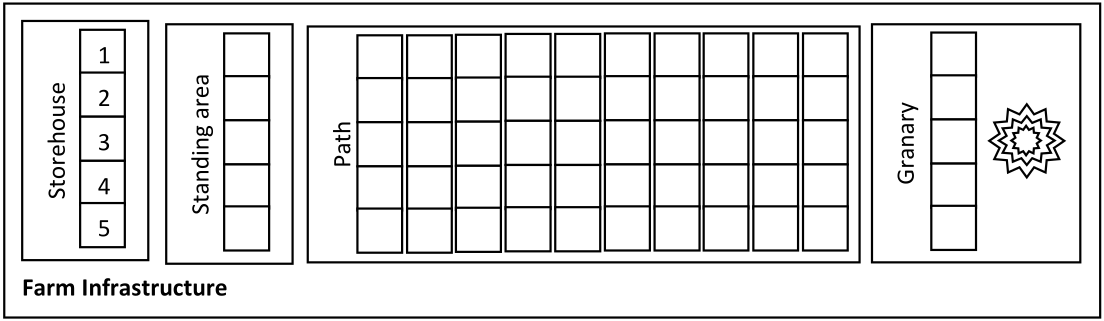
\includegraphics[width=\linewidth]{img/Design_FI.png}
%   \end{minipage}%
%   \caption{Visual representation of the farm, taken from \cite{assign}.}
%   \label{Design_FI}
% \end{figure} 

%\texttt{java -cp <userdir>/build/classes fi.FarmInfrastructure}

\newpage
\section{IoT, Kafka and Connected Devices} %%%%%%%%%%%%%%%%%%%%%%%%%%%%%%%%%%%%%%%%%%%%%%%%%%%%%%%%%%%%%%%%%%%%%%%%%%%%%%%%%%%%%%%%%%%%%%%%%%%%%%%%%%%%%%%%%%%%%

Internet of Things (IoT) is becoming an increasing topic of interest among technology giants and business communities.
IoT Components are interconnected devices over a network, which are embedded with sensors, software and smart applications so they can collect and exchange data 
with each other or with cloud / data centers.

One of the areas in which IoT is paving its way is the connected vehicles. 
According to Gartner predictions \cite{gartner}, by this year there should be about a quarter-billion connected vehicles on the road, which are more automated, 
providing new in-vehicle services such as enhanced navigation system, real-time traffic updates, weather alerts and integration with monitoring dashboards. 
In order to process the data generated by IoT connected vehicles, data is streamed to central processors usually located in the cloud. 
The collected information can be analysed and data can be extracted and transformed to the final result, which can be sent back to the vehicle or to a monitoring dashboard. 

In this project we explore a hypothetical use case where communication between devices (or entities) is done through Kafka.
Apache Kafka \cite{kafka} is high-throughput distributed messaging system in which multiple producers send data to Kafka cluster and which in turn serves them to consumers. 
It is a distributed, partitioned, replicated commit log service.
The Java application we developed and that is described in this report is a simplified version of an IoT data processing and monitoring application for connected
vehicles, aimed to to explore Kafka capabilities for messaging between entities.

\subsection{The Data} %%%%%%%%%%%%%%%%%%%%%%%%%%%%%%%%%%%%%%

As having actual connected vehicles with processing units capable of collecting car data and transmitting it to other entities was out of the scope of the project, 
this is simulated through a simple text file containing 1 transmission (or message) per line.
This data file with the name of \texttt{CAR.TXT} is placed under a specific directory and is read by our system for processing.

In order to dynamically generate such source data, we developed a small script in Python that receives as parameters the number of cars to be simulated and the 
total number of messages to be generated from those cars and stored in the text file.
The script is called \texttt{generateCAR.py} and is placed in the scripts package inside our project.
By default, it creates 10 different cars and writes 100 messages, but these numbers can be easily modified inside the script. 

We used a random-based approach to generate each aspect of a message.
Unique register codes are created to represent vehicles, as well as their status and speeds.
Message types are not generated with a specific pattern, but we made it far more likely to generate a message of type HEARTBEAT (see section \ref{messages}) 
than of any other type.

%A car is characterized by a register code NN-XX-NN, where N is a number between 0 and 9 and X is a letter from the alphabet in uppercase, so we merely compute 
%random numbers within that range and random indexes from 0 to the size of the used alphabet and build register codes. 
%These codes are validated (ensured to be unique) before adding them to an array of car codes.
%Message types are also determined randomly, although some types are made more likely than others, as well as message timestamps, car speeds and car status values.
%The maximum period between messages is of 5 seconds, although this number is also easily configurable inside the script.
%The maximum car speed is of 150 Km per hour and it is assumed that they are only allowed to drive at up to 120 Km per hour.

\subsection{The Messages} \label{messages} %%%%%%%%%%%%%%%%%

Messages can be of 1 of 3 types, each with a specific purpose and format:

\vspace{-10pt}
\begin{itemize}[noitemsep]
  \item HEARTBEAT - the simplest type of message meant to notify the system that the car is still connected. \\ Format: $|$ car\_reg $|$ timestamp $|$ 00 $|$
  \item SPEED - message meant to inform the system about the current speed of the car. This allows the system to determine whether the car is going under the speed limit or not and trigger an alarm if necessary. \\ Format: $|$ car\_reg $|$ timestamp $|$ 01 $|$ speed $|$
  \item STATUS - messages meant to detect whether the smart sensor detects any malfunction. This in theory could help the system provide or suggest a solution for the malfunction to the car driver considering the entire network of connected vehicles. \\ Format: $|$ car\_reg $|$ timestamp $|$ 02 $|$ status $|$
\end{itemize}
\vspace{-10pt}
The car\_reg corresponds to the register code of each vehicle and the timestamp corresponds to the time instance when the message was created, the remaining 
elements are self explanatory.
As we will see, each message type is treated differently both in their purpose and in the care with which their transmission is done. \\
  
$|$ 45-SH-72 $|$ 1586183268975 $|$ 02 $|$ OK $|$

$|$ 28-MC-82 $|$ 1586183269976 $|$ 02 $|$ OK $|$

$|$ 42-UW-71 $|$ 1586183272978 $|$ 00 $|$

$|$ 73-FD-20 $|$ 1586183273979 $|$ 00 $|$

$|$ 28-MC-82 $|$ 1586183274980 $|$ 01 $|$ 20 $|$

$|$ 55-LZ-42 $|$ 1586183276981 $|$ 00 $|$

$|$ 64-IY-98 $|$ 1586183281986 $|$ 00 $|$

$|$ 45-SH-72 $|$ 1586183286989 $|$ 00 $|$

$|$ 42-UW-71 $|$ 1586183311005 $|$ 00 $|$

$|$ 80-DE-01 $|$ 1586183315006 $|$ 00 $|$

$|$ 30-UU-59 $|$ 1586183319009 $|$ 00 $|$

$|$ 78-ST-77 $|$ 1586183324009 $|$ 00 $|$

$|$ 28-MC-82 $|$ 1586183325011 $|$ 02 $|$ KO $|$

$|$ 30-UU-59 $|$ 1586183327012 $|$ 01 $|$ 0 $|$

$|$ 73-FD-20 $|$ 1586183328012 $|$ 01 $|$ 130 $|$

Example of a portion of the \texttt{CAR.TXT} file.

\newpage 
\section{System Architecture} %%%%%%%%%%%%%%%%%%%%%%%%%%%%%%%%%%%%%%%%%%%%%%%%%%%%%%%%%%%%%%%%%%%%%%%%%%%%%%%%%%%%%%%%%%%%%%%%%%%%%%%%%%%%%%%%%%%%%%%%%%%%%%%%%%

Modular architecture is very appealing for IoT solutions, as it offers a way to manage the complexity of a problem by breaking it down to smaller and more 
easily manageable modules.
Plus, IoT components are constantly changing, so limiting the effects of such organic-like transformations to individual modules allows developers to keep in 
control of the system's growth.

Software applications are embracing distributed, decentralized, real time and on-the-cloud as the new norm. 
They are focused on providing real service rather than just being obsessed on lists of features.
This is what drives the increase in awareness for the importance of modularity in software development.
And this is partly what was meant to be explored in this assignment.
So in this chapter we focus on presenting the interacting entities of our vehicle supervising system and the components that constitute their functionality.

\subsection{Entities} %%%%%%%%%%%%%%%%%%%%%%%%%%%%%%%%%%%%%%

There are 4 entities, each with its own responsibilities.
These entities simulate the management of the car network, with representative features of what could be accomplished by a fully implemented version.
Following is their description and a simple block diagram in Figure \ref{BlockDiagram}.

\vspace{-10pt}
\begin{itemize}[noitemsep]
  \item CollectEntity - its role is to collect data from connected vehicles (represented by \texttt{CAR.TXT}) and produce messages to the other entities with the gathered information (through communication channels established \textit{a priori} and explained in chapter \ref{infrastructure}).
  \item ReportEntity - as the name states, this entity is responsible for reporting all that is transmitted by CollectEntity, writting it to \texttt{REPORT.TXT}.
  \item BatchEntity - Batch's role is to make possible the computation of any relevant metrics and calculations related to the information collected; in our case it merely accomplishes the same as ReportEntity, writting results to \texttt{BATCH.TXT}.
  \item AlarmEntity - its role is to trigger alarms and present them to the system user when some relevant event occurs; in our case alarms are triggered when a car surpasses the predefined speed limit of 120 Km/h; all alarms are written to \texttt{ALARM.TXT}.
\end{itemize}
\vspace{-10pt}

\begin{figure}[H]
  \centering
  \begin{minipage}{\textwidth}
    \centering
    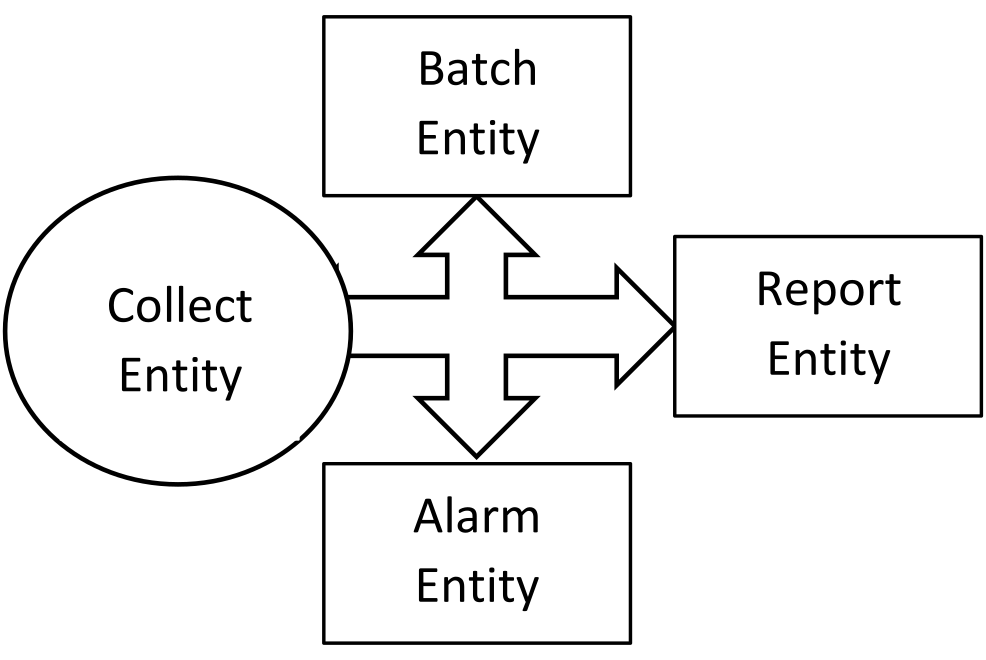
\includegraphics[width=.4\linewidth]{img/BlockDiagram.png}
  \end{minipage}%
  \caption{Basic block diagram for the system, taken from \cite{assign}.}
  \label{BlockDiagram}
\end{figure} 

\subsection{Components} %%%%%%%%%%%%%%%%%%%%%%%%%%%%%%%%%%%%

The Java application is organized with packages.
Each package contains a set of files with common natures so that managing source code is made easy.
The "data" package contains both the input (CAR.TXT) and the output data (REPORT.TXT, BATCH.TXT and ALARM.TXT).
The "entities" package contains every entity class.
The "scripts" package holds project scripts, including the Kafka initialization and deletion scripts and the CAR.TXT file generation script.

The "message" package contains all classes related to the messages sent through Kafka; here we have the Message class, with all that was described in section 
\ref{messages}, and our implementations of the serializer and deserializer classes of Message instances.
Kafka has serialization classes available for non-structured data such as regular integers or strings, but we intended to send a structured message for greater 
usability, so implementing a serialization process for such structure was required in order to transmit data through Kafka.

Finally, the "kafkaUtils" package provides Kafka utilities such as EntityAction.
This interface, implemented by all consumer entities, ensures that such entities have means to process Kafka messages in a predefined format by defining the 
method \textit{processMessage()}.
This method receives the identifier of the consumer that is going to process the current message, the topic that the message belongs to and the key-value pair of 
the message.

The package also contains our implementations of Kafka Consumers and Producers.
Kafka is explained in greater detail in chapter \ref{infrastructure}, however a simple way of understanding producers and consumers in Kafka is to see them as 
the components responsible for creating messages that can be sent via Kafka topics and sending them, and for subscribing to topics and receiving messages from them,
respectively.
By implementing our own versions of such components, we gain greater control over their configurations and functionalities.
The Producer class supports 3 message sending methods:
\vspace{-10pt}
\begin{itemize}[noitemsep]
  \item \textit{fireAndForget()} - where messages can be lost or arrive reordered on the consumer side.
  \item \textit{sendAsync()} - where the producer asynchronously awaits for a delivery confirmation with the use of callbacks.
  \item \textit{sendSync()} - where the producer waits for a delivery confirmation before proceeding to processing another message, ensuring the correct order on the consumer side.
\end{itemize}
\vspace{-10pt}
Producer also has an inner class called ProducerCallback that, as the name suggests, deals with the callbacks related to the executions of the method \textit{sendAsync()}.
The Consumer class on the other hand works as a java thread by implementing the Runnable interface.
Once instantiated, it listens to the topics where it is subscribed and processes arriving messages by calling \textit{processMessage()}.
Each consumer has an instance of RebalanceListener, our implementation of Kafka's ConsumerRebalanceListener for partition management.
This listener is explained in greater detail in section \ref{topics}.

\begin{figure}[H]
  \centering
  \begin{minipage}{\textwidth}
    \centering
    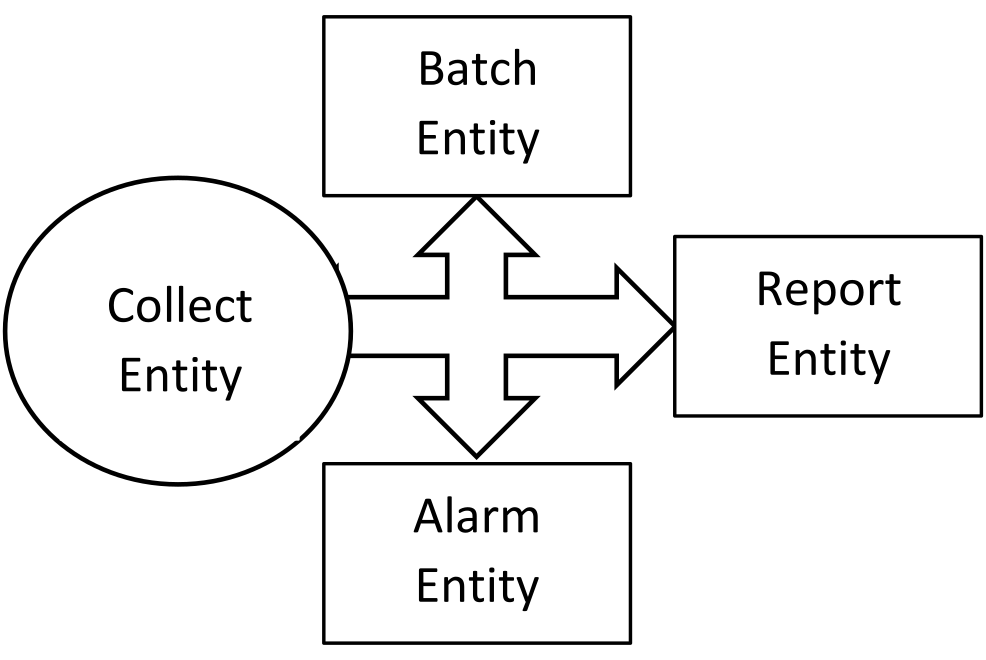
\includegraphics[width=.5\linewidth]{img/BlockDiagram.png}
  \end{minipage}%
  \caption{Java application's class diagram.}
  \label{ClassDiagram}
\end{figure} 

Figure \ref{ClassDiagram} presents the project's class diagram with the relations between components.
In order to more easily visualize interactions between entities, we designed an interaction diagram as well, present in Figure \ref{InteractionDiagram}.

\begin{figure}[H]
  \centering
  \begin{minipage}{\textwidth}
    \centering
    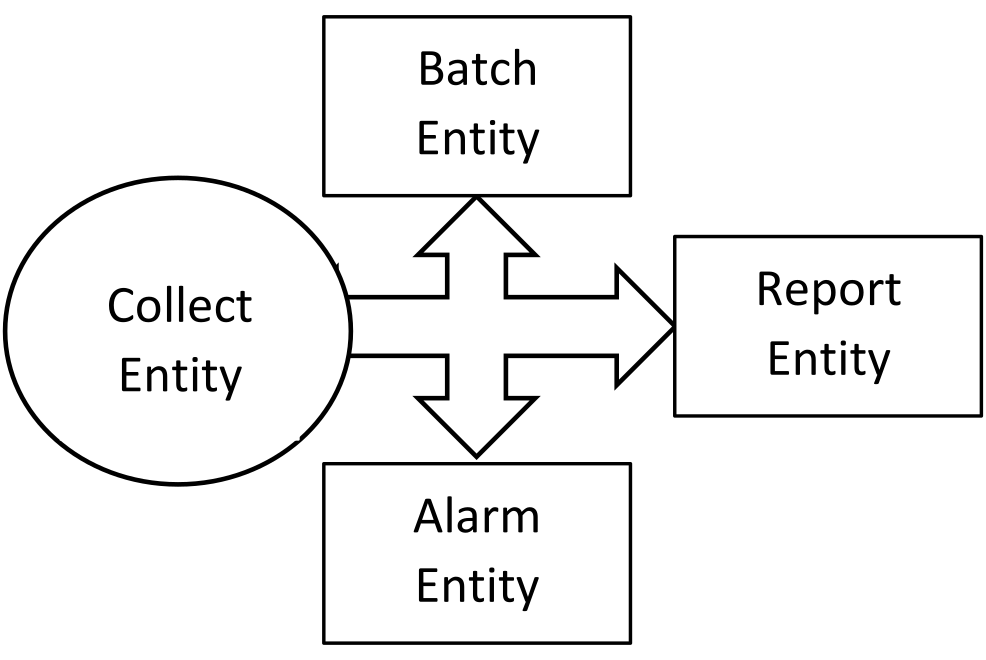
\includegraphics[width=.5\linewidth]{img/BlockDiagram.png}
  \end{minipage}%
  \caption{Entities interaction diagram.}
  \label{InteractionDiagram}
\end{figure} 

\subsection{User Interface} %%%%%%%%%%%%%%%%%%%%%%%%%%%%%%%%

...

\newpage
\section{Kafka Infrastructure} \label{infrastructure} %%%%%%%%%%%%%%%%%%%%%%%%%%%%%%%%%%%%%%%%%%%%%%%%%%%%%%%%%%%%%%%%%%%%%%%%%%%%%%%%%%%%%%%%%%%%%%%%%%%%%%%%%%

As a distributed streaming platform, Apache Kafka has 3 main capabilities: publish and subscribe to record streams, similarly to a message queue or 
messaging system; store those record streams in a fault-tolerant way; process streams of records as they occur. 
Its general use is for building real-time streaming data pipelines to establish communication between applications, and building real-time streaming applications 
to transform and react to streams of data.

For our specific case, the messaging system scenario seemed the most appropriate.
As stated in their online documentation \cite{kafka}, normally these type of systems follow 2 possible models: message queueing or publish-subscribe. 
The queue model is characterized by a pool of consumers that read from the messaging server and each record goes to one of the consumers; 
this has several positive aspects such as allowing the division of the records in a balanced fashion by the registered consumers and enabling the processing rate 
and power to scale; on the other hand, being a queue, when a record is processed it may not be reprocessed.
Comparatively, the publish-subscribe model is characterized by broadcasting each record to all registered consumers; this broadcasting feature can be seen as a 
positive aspect, but is counterweighted by the fact that there is no way to scale the process, since every message is sent to every consumer.

With this in mind, we established Kafka's infrastructure as the message system and the backbone for the entire system, making use of both models metioned above.
The usage of this platform was not only a constraint in the proposed assignment, but was also justified by our own personal analysis that showed that Kafka is a 
solution complete enough for our purposes and guarantees a number of quality metrics that were found important.
It was these metrics we explored during development in order to understand their influence on the quality attributes of a system with a standard IoT architecture. 

\subsection{Initialization and Destruction Scripts} %%%%%%%%

Obviously, to use this platform we first needed to instantiate the services and infrastructure composing Apache Kafka. 
To do so, we had 2 approaches: use the instantiation scripts provided with the source code available online \cite{kafka} or use docker as a middleware 
framework that would enable us to abstract the the instantiation process and use Kafka in a container. 
We chose the former option, which requested more work from our side but enabled us to instantiate the platform with more precision and control.

Manually running each necessary command was obviously out of question.
The solution was to develop 2 scripts to automate both the creation and deletion of the infrastructure necessary for this project. 
These scripts are available together with the source code, in the package folder \texttt{scripts}.

The initialization script is the first action to be executed when the project is ran.
Also, as you might guess, the deletion script is the last thing to be executed before the system is terminated.
In relation to \textit{initKafka.sh}, the initialization script, it is responsible for: starting Zookeeper, the entity in charge of managing the Kafka Brokers;
initializing the Kafka Brokers themselves, entities with the logic of the platform, for service providing (3 brokers are deployed); creating the necessary Kafka Topics.
The final order of actions performed is:
\vspace{-10pt}
\begin{enumerate} [noitemsep]
  \item Instantiate Zookeeper
  \item Instantiate Kafka Brokers
  \item Store process IDs of the Kafka Brokers in a auxiliary file
  \item Create necessary topics for this project
\end{enumerate}
\vspace{-10pt}
In relations to \textit{deleteKafka.sh}, the deletion script, its responsibility is to kill the processes previously stored in the auxiliary files and delete 
the logs generated by the same processes.
The final order of actions performed is:
\vspace{-10pt}
\begin{enumerate} [noitemsep]
  \item Fetch process IDs from the auxiliary file
  \item Kill the fetched processes
  \item Delete the generated logs
\end{enumerate}
\vspace{-10pt}

\subsection{Topics and Constraints} \label{topics} %%%%%%%%%
To establish constraints to the infrastructure consequently to the project, we had 3 methods, either in the definition of properties for the consumers, in the definition of the producers or in the definition of properties for the topics themselves.

For this project it was established that there should only exist 3 topics, the \textit{BatchTopic}, \textit{ReportTopic} and the \textit{AlarmTopic}, each one with the objective of establishing communication between the \textit{CollectEntity} and the \textit{BatchEntity}, \textit{ReportEntity} and \textit{AlarmEntity}, respectively.

As already mentioned, there are three different types of messages, and all types should be sent to every one of the topics. This condition is quite relevant since this means that the properties and conditions assured in shared resources across message types, such as the topics, will be dictated by the most restricting message type. The higher restrictions on a given constraint can be defined by different message types, since each message type as a different set of constraints. Those constrains are:

\begin{multicols}{3}
  \begin{itemize}
    \item HEARTBEAT
    \newline - can be lost
    \newline - can be reordered
    \newline - can be reprocessed
  \end{itemize}

  \columnbreak

  \begin{itemize}
    \item SPEED
    \newline - can be lost
    \newline - cannot be reordered
    \newline - cannot be reprocessed
  \end{itemize}

  \columnbreak

  \begin{itemize}
    \item STATUS
    \newline - cannot be lost
    \newline - cannot be reordered
    \newline - can be reprocessed
  \end{itemize}
\end{multicols}

To ensure these constraints, efforts can be made in several points along the data flow.

\subsubsection{Message Lost}\label{lost}
This constraint needed only to be assure to the status type message. After some research we found that there were specific properties for the producer and topics to ensure the message persistence. Additionally a specific consumer behavior was taken in consideration to further assure a lossless data flow.

From the producer side, the \textit{acks} property was the one that we found to be the most relevant for this aspect. This property is related to the way the kafka leader considers the send request complete. There are three option, the leader when receiving a request to store a message immediately considers the request complete, not making sure the message was persisted in its logs nor requesting the acknowledge of any of its followers; another option is to assure the message is persisted in the leader itself, returning request complete without requesting the acknowledge of its followers; the last and most secure way is to return only after the leader and all its followers acknowledges the persistence of the message. The codification of this modes is made by assigning "0" to no acknowledges, "1" to only the leader's acknowledge and "-1"/"all" to the acknowledge of every entity involved. We ended up setting the \textit{acks} property the "0" mode to the HEARTBEAT message type, since it can be lost and "all" mode for the STATUS message type since it cannot be lost. For the SPEED message type, although it can be lost, the \textit{acks} mode was set to "all" due to another constraint(see Section \ref{reprocessing}).Additionally, for the HEARTBEAT and SPEED status we used the \texttt{fire and forget} method of sending message, since the Kafka response was not important to assert if the persistance of the message was successful or not; comparatively, for the STATUS type message we went the last effort and used the \texttt{synchronous} method, which enabled us to wait for the Kafka response, and in case of an error we re-sent the message to assure the correct persistance of the message in the Kafka system.

From the topics point of view, the replication factor is quite important in a no-message-loss scenario, since it is mandatory that the message is stored not in a single place, since in that fashion a single point of failure would be created and in the event of that single machine containing critical messages crashing, all those messages would be lost since there were no backups. For that reason replication is a must in a critical scenario. We ended up settling in a replication factor of 3, which we considered to be a satisfactory number for our context.

Lastly, in the consumer side, we noticed that it was desirable for our system to manually commit the offsets for us to have a greater control over this aspect. This option enabled us to decide were we wanted to commit the processed offsets, either before the message processing or after the message processing. To compare both options, the first one, were we commit before processing the data, this scenario makes allows the loss of some messages, since it can happen that the consumer fetches messages from the Kafka system, commits the offsets and immediately crashes, not processing those messages, loosing them; on the other hand, if the offset commit is after the message processing, this may cause message reprocessing since in the case the consumer fetches messages from the Kafka system processes them and crashes right after, not committing them and enabling reprocessing. This was all taken in consideration but was submitted to another constraint which made us implement this offset commit in another fashion. See Section \ref{reprocessing}.

% With all of these efforts we minimized the probabilities of losing a message.

\subsubsection{Message Reordering}
For this constraint we found two properties in the producer side as well as a specific way of sending the message that seemed enough to handle this reordering aspect, and through test showed to be true.

Those properties were the \textit{retries} and \textit{max.in.flight.requests.per.connection}. The retries property establishes a maximum number of retries per send request. The max.in.flight.requests.\\per.connection, as the name implies, establishes a maximum number of parallel active connections to the Kafka leader. These two properties when combined in a specific way can minimize or even neutralize the reordering probability. The values these properties have by default, which are 2147483647 for the retries and 5 for the max.in.flight.requests.per.connection allow the messages to be reordered, and to illustrate that a brief example will be given. Suppose that we send a message but the Kafka leader takes some time to respond and in that time a new connection with another message is also produced, in the case the first message response is unsuccessful and the one is successful, the first one due to the retries established will re-send the request, changing the intended order of the messages. To prevent this case, we decided that for both the SPEED and STATUS message types, the ones were the order is mandatory, we assigned the value "1" to max.in.flight.requests.per.connection, neutralizing the reordering possibility.

In relation to the sending message message, we also took in consideration the fact that our Kafka system was partitioned, which meant that if not specified, Kafka itself would distribute the messages in a balanced fashion across all available partitions, this would cause the order to also be lost. To neutralize that possibility, all messages of SPEED and STATUS type were produces to a specific partition, in our case, both to partition 0 since as stated by the project description, HEARTBEAT messages are produced in a much larger scale in comparison top the other two message types, so HEARTBEAT is the message type that makes sense in partitioning, as already stated in this section.

\subsubsection{Message Reprocessing}\label{reprocessing}
Lastly, in relation to the reprocessing constraint, after some research we settled on one property on the producer side and mainly a consumer side behavior we needed to adopt.

In relation to the producer side property we found the \textit{enable.idempotence} property, which when enabled will assure that the producer only writes one copy of the message. Otherwise, due to retries, more than one copy can be persisted which can cause reprocessing of the message. SPEED message type was the one that required not to be reprocessed, and for that reason was the one were this property was enabled. For the correct operation of this property, other properties are affected, such as the max.in.flight.requests.per.connection that need to be less or equal to 5, the retries need to be higher than 0 and acks need to be "all". This last internal constraint was the reason the acks property was set to "all" in the SPEED message type(as mentioned in Section \ref{lost}), which decreases the message loss probability but remains possible due to the fire and forget method.

Lastly, for the consumers efforts, we found that the usage of a \texttt{Rebalance Listener} was necessary. \texttt{Rebalance Listener} is an entity which follows a Kafka defined behavior(interface), that enables the injection of code in two specific events when assign to a consumer. Those events are in case new partitions or topics are assigned to the consumer or when partitions or topics are revoked from that consumer due to the consumer not signalling it is alive for a long time or a new consumer being added in the consumer group. Obviously we were more interested in the last event, where partitions and topics are removed from the consumer, since that enabled us to commit the latest processed offsets.

A note need to be made in relation to the consumption strategy we adopted. when analyzing this we found two options, either we instantiated 3 different consumer groups per topic with one or more consumers assigned to them to make possible a grainer control over the constraints assigned to each message type or one consumer group per topic with the most restricting constraints with one or more consumers assigned to it. The first option of 3 distinct consumer groups per topic didn't seemed to be the most correct nor the most efficient, since each message was going to be consumed 2 times more just to make possible the separation of messages in the three available types. This from our point of view is not scalable, since if there were 100 messages types we would need 100 consumer groups and creates unnecessary overhead.

For that reason we implemented only one consumer group per topic which deals with all messages types in a efficient way. Given the fact that every topic may contain every message type and existing only one consumer group per topic, the order constraint of the SPEED message type meant that we needed to implement the Rebalance Listener to every consumer of every consumer group.

\newpage
\section{Additional Remarks} %%%%%%%%%%%%%%%%%%%%%%%%%%%%%%%%%%%%%%%%%%%%%%%%%%%%%%%%%%%%%%%%%%%%%%%%%%%%%%%%%%%%%%%%%%%%%%%%%%%%%%%%%%%%%%%%%%%%%%%%%%%%%%%%%%%

\subsection{Documentation} %%%%%%%%%%%%%%%%%%%%%%%%%%%%%%%%%

Our attitude towards the developed code was to ensure it could be applied to other similar scenarios and reused in systems intended to be deployed in real scenarios.
With this in mind, we took great care with regards to code readability.
By maintaining a code style equal throughout the project and defining intuitive and self-explaining variable and method names, we made the code easy to understand
by someone already contextualized with Kafka.

Nevertheless, we wanted to make sure this was also true to someone looking at our project for the first time, so we resorted to the well-known Javadoc 
\cite{javadoc} tool to manage all code documentation.
Comments were also added in key points throughout the code, including the scripts.

\subsection{Assignment Contributions} %%%%%%%%%%%%%%%%%%%%%%

As the entire development phase took place in a time where on-site cooperation was not possible, we resorted to online communication platforms to debate decisions
and discuss difficulties.
Team scheduling allowed us to work on the project simultaneously, so no member suffered from unbalanced workloads.
The dimension of the project did not appeal to the usage of repository pull requests and other synchronization tools.
However, each small solution was verified and agreed by both team members.

Having said this, it is difficult to isolate what each member actually implemented, as the influence of both is present in all components.
Nevertheless, one might say that each had stronger responsibilities on a set of project aspects:
Filipe took care of the execution of the individual Java processes and of the Shell scripts, while João developed the Kafka-related classes such as Consumer,
Producer and EntityAction; Filipe developed the Python script for generation of \texttt{CAR.TXT}, while João developed the Shell scripts for Kafka initialization 
and deletion; each implemented 2 entities and each wrote a portion of this report; Filipe made sure everything was coherent throughout the report and the code 
documentation, while João solved the most critical issues regarding the configuration of the topics.
In terms of work percentage, we believe it was about 50\% for each student.

\newpage
\section*{Conclusions} %%%%%%%%%%%%%%%%%%%%%%%%%%%%%%%%%%%%%%%%%%%%%%%%%%%%%%%%%%%%%%%%%%%%%%%%%%%%%%%%%%%%%%%%%%%%%%%%%%%%%%%%%%%%%%%%%%%%%%%%%%%%%%%%%%%%%%%%%

........................

\begin{thebibliography}{9} %%%%%%%%%%%%%%%%%%%%%%%%%%%%%%%%%%%%%%%%%%%%%%%%%%%%%%%%%%%%%%%%%%%%%%%%%%%%%%%%%%%%%%%%%%%%%%%%%%%%%%%%%%%%%%%%%%%%%%%%%%%%%%%%%%%%%
  \bibliographystyle{Science}

  \bibitem{assign}
    Óscar Pereira,
    \textit{SA: Practical Assignment no.2},
    University of Aveiro,
    2019/20.
  
  \bibitem{gartner}
    Smarter With Gartner,
    \textit{Staying on Track with Connected Car Security},
    \url{https://www.gartner.com/smarterwithgartner/staying-on-track-with-connected-car-security/},
    accessed in April 2020.

  \bibitem{kafka}
    Apache Kafka,
    \textit{Apache Kafka: A Distributed Streaming Platform},
    \url{https://kafka.apache.org/},
    acessed in April 2020.

   \bibitem{javadoc}
    Oracle,
    \textit{Javadoc Technology},
    \url{https://docs.oracle.com/javase/8/docs/technotes/guides/javadoc/index.html},
    accessed in April 2020.


  % \bibitem{uml}
  %   Object Management Group,
  %   \textit{What is UML},
  %   \url{https://www.uml.org/what-is-uml.htm},
  %   accessed in March 2020.
    
 

\end{thebibliography}

\clearpage

\end{document}




















